

\section{Изучение материала}
В ходе выполнения преддипломной практики были изучены следующие источники:


В источниках был встречен \textit{метод наименьших квадратов по центрам интервалов}.
Метод заключается в следующем:
пусть имеется $\mu_i$ - номер полуинтервала, в который попало очередное наблюдение $y_i$. Ему соответствует полуинтервал $\nu_{\mu_i}$ (см ф.\ref{eq13}), т.е. полуинтервал:
\begin{eqnarray}
    (a_{\nu_{\mu_i}},a_{\nu_{\mu_i}+1}],
\end{eqnarray}
(считаем что $a_1<y_i<a_{k-1}, i=\overline{1,n}$).

Найдем центральную точку этого интервала, т.е. точку
\begin{eqnarray}
    \check{y_i} = \frac{a_{\nu_{\mu_i}} + a_{\nu_{\mu_i}+1}}{2}
\end{eqnarray}

Построим для всех значений функции регрессии $y_i$ значения $\check{y_i}$.
Будем использовать в качестве значений функции регрессии полученные значений, а в качестве регрессоров $x_i$ и построим МНК оценки параметров $\beta$.

\newpage
\section{Реализация оценок}
Описанные оценки были построены путем наследования от исходных оценок и переопределения соответствуюего метода fit(). 
\begin{Verbatim}[fontsize=\scriptsize]
class ApproximationGEMModelNaive(ApproximationGEMModelRedesigned):
    def fit(self):
        self.classify()

        def ex_generator(mu_data):
            for i in range(0, self.endogen.size):
                if mu_data[i] is None:
                    continue
                a_mu_i_plus_1 = mu_data[i] * Defines.INTERVAL_LENGTH
                a_mu_i = mu_data[i] * Defines.INTERVAL_LENGTH - Defines.INTERVAL_LENGTH
                yield (a_mu_i_plus_1 + a_mu_i) / 2

        naive_ex_data_positive = np.fromiter(ex_generator(self._np_freq_positive), float)
        naive_ex_data_negative = np.fromiter(ex_generator(self._np_freq_negative), float)

        naive_ex_data_full = np.append(naive_ex_data_positive, naive_ex_data_negative)

        z, resid, rank, sigma = np.linalg.lstsq(self.exogen, naive_ex_data_full, rcond=None)
        return z
\end{Verbatim}

\newpage
\section{Компьютерные эксперименты}
\subsection{Параметры модели и оценок}
\begin{center}
    \begin{tabular}{|p{5cm}|p{5cm}|}
        \hline
        \multicolumn{2}{|c|}{Параметры программы} \\
        \hline
        Переменная&значение\\
        \hline
        Размер выборки $N$& 1000\\
        \hline
        Доля выбросов $\widetilde{\varepsilon}$& 0.8\\
        \hline
        Параметры регрессии $\beta$& $(90,4)$\\
        \hline
        Регрессоры $x_i$ & $\sim U(-5,5)$\\
        \hline
        $\varepsilon_i$&$\sim N(0,16)$\\
        \hline
        $\eta_i$&$\sim N(100,100)$\\
        \hline
        Величина $K$ из пункта 2.3 курсового проекта &$10$\\
        \hline
    \end{tabular},
\end{center}

\subsection{Сравнительный анализ построенной оценки с альтернативной}
Если сравнить вариации оценок построенные на рис.\ref{pic1}, можно увидеть, что оценки, построенные по методу, предложенному в курсовом проекте, показывают лучшие результаты
\begin{figure}[h!]
    \centering
    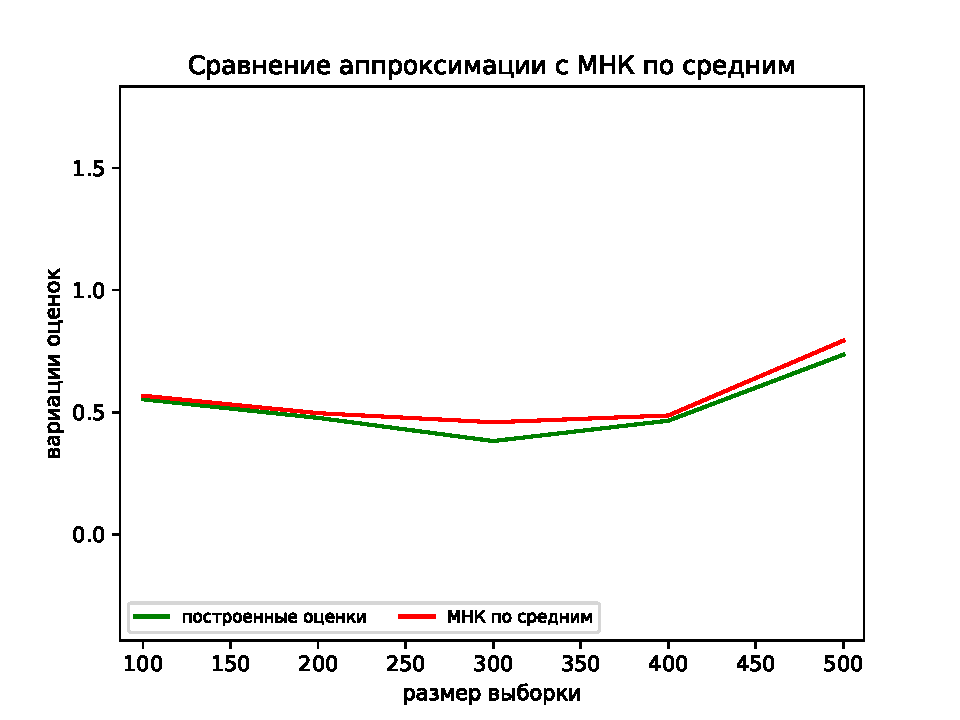
\includegraphics[width=100mm]{../images/OLS_GEM.pdf}
    \caption{Сравнение вариаций оценок\label{overflow}}
    \label{pic1}
\end{figure}

\newpage
\subsection{Дополнительные эксперименты}
\subsubsection{Эксперименты с переклассификацией выборки}
В построенном методе использовался метод $K$-соседей.

На первом этапе для каждого $x_i$ имели класс $\mu_i$: т.е. пару $(x_i,\mu_i)$.
Далее пытались переклассифицировать выборку. 
Для этого строилась новую выборка такого же объема $N$.
Проходились по каждому элементу $(x_i, \mu_i)$ выборки и для этого наблюдения строилось новое:
\begin{eqnarray}
    (x_i, \check{\mu}_i),
\end{eqnarray}
где $\check{\mu}_i$ получен по методу $K$-соседей.\hfill\break
\begin{eqnarray}
    \check{\mu}_i = \arg\max_j \sum_{k \in V_i,~k\neq i} \delta_{\check{\mu}_k j}~,
\end{eqnarray}
где $V_i$ множество индексов $l$ первых $K$ векторов $x_l$, отсортированных по возрастанию расстояния до вектора $x_i$.

После переклассификации выборки, применяли к ней функцию правдоподобия из уравнений (\ref{eq22}-\ref{eq23}), только теперь с использованием новых классов $\check{\mu}_i$ вместо $\mu_i$. 
Аналогично максимизировали ее и находили новую оценку параметров $\hat{\beta}$.

В ходе преддипломной практики были построены эксперименты с изменением величины K для метода $K$-ближайших соседей, используемого в переклассификации. Параметры использовались такие же, как в ранее приведенной таблице.
\begin{figure}[h!]
    \centering
    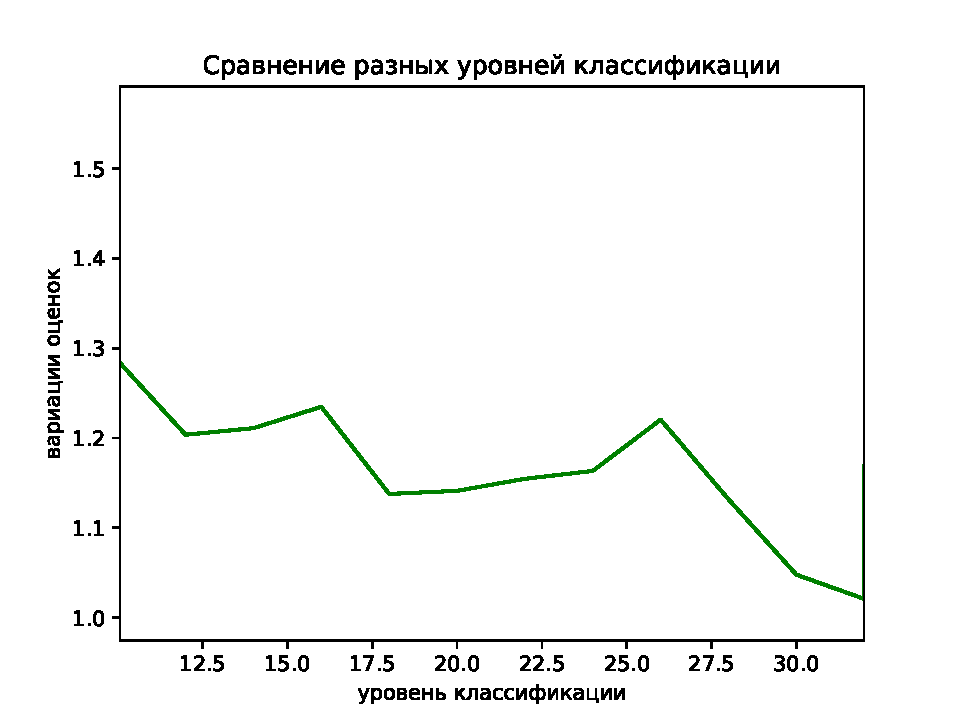
\includegraphics[width=100mm]{../images/different_recl_level.pdf}
    \caption{Зависимость от K, упомянотого в пункте 2.3 курсового проекта\label{overflow}}
    \label{pic1}
\end{figure}

В результате получилось, что при увеличинии константы K точность оценки параметров растёт. Но в ходе экспериментов оказалось, что нельзя делать константу К сильно большой: в противном случае точность аппроксимации падает.

Были проведены эксперименты, когда использовалась вышеописанная переклассификация и когда нет. При этом на каждой итерации выборка увеличивалась. 
\begin{figure}[h!]
    \centering
    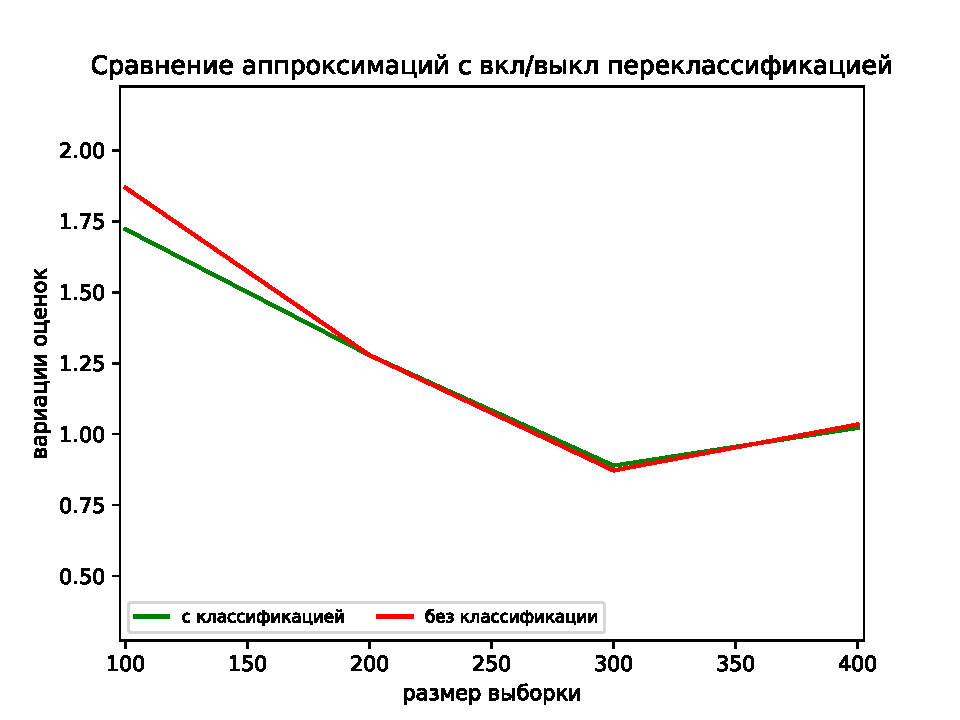
\includegraphics[width=100mm]{../images/on_off_recl.pdf}
    \caption{Сравнение вариаций оценок когда используется и не используется переклассификация\label{overflow}}
    \label{pic2}
\end{figure}

\newpage

\subsubsection{Использование полиномиальной регрессии}
Введем теперь модель полиномиальной регрессии.

\begin{equation}
    \begin{array}{c}
        \label{eq28}y_i=\beta_0+\beta_1 x_{i1}^1+\beta_2 x_{i2}^2+\dots+\beta_n x_{in}^n+\varepsilon_i, i=\overline{1,N},\\
        y_i = \sum\limits_{l=1}^{n} x_{il}^{l-1} + \varepsilon_i, i=\overline{1,N},\\
        y_i= f(x_i,\beta)+\varepsilon_i,\\
        f(x_i,\beta)=\beta_0+\beta_1 x_{i1}^1+\beta_2 x_{i2}^2+\dots+\beta_n x_{in}^n
    \end{array}
\end{equation}

Построенные по формуле (\ref{eq28}) $y_i$ также как и в случае линейно регрессии будем использовать в формуле (\ref{eq3}):
\begin{eqnarray}
    y_i^{\widetilde{\varepsilon}}=(\xi_i)y_i+ (1-\xi_i)\eta_i,
\end{eqnarray}

Несложно заметить, что построенные в курсовом проекте оценки никак не зависят от регрессоров, они выступают лишь как параметры, поэтому можно моделировать полиномиальную регрессию и применить к ней описанный метод.

Были построены графики, схожие с рис.\ref{pic2}. В итоге получился такой график:
\begin{figure}[h!]
    \centering
    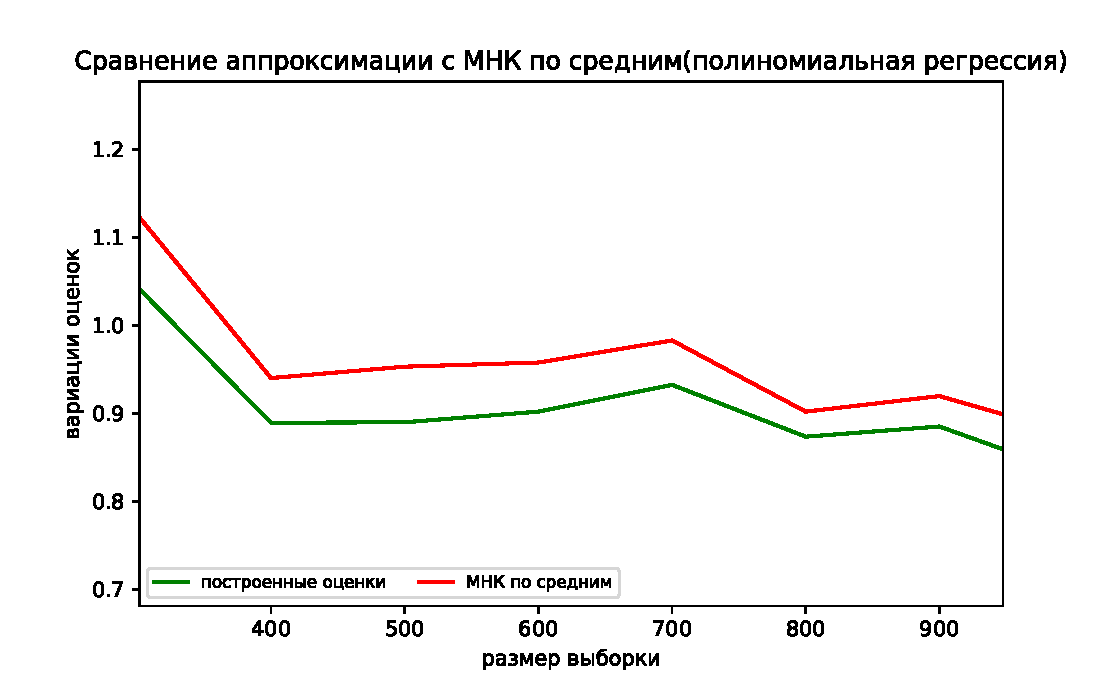
\includegraphics[width=150mm]{../images/polynomial.pdf}
    \caption{Аппроскимация параметров в случае полиномиальной регрессии\label{overflow}}
    \label{pic1}
\end{figure}

Видим, что обе модели имеют схожее поведение при изменении объема выборки, но построенные новые оценки стабильно показывают лучший результат.